% Options for packages loaded elsewhere
\PassOptionsToPackage{unicode}{hyperref}
\PassOptionsToPackage{hyphens}{url}
%
\documentclass[
]{article}
\usepackage{amsmath,amssymb}
\usepackage{iftex}
\usepackage{CTEX}
\ifPDFTeX
  \usepackage[T1]{fontenc}
  \usepackage[utf8]{inputenc}
  \usepackage{textcomp} % provide euro and other symbols
\else % if luatex or xetex
  \usepackage{unicode-math} % this also loads fontspec
  \defaultfontfeatures{Scale=MatchLowercase}
  \defaultfontfeatures[\rmfamily]{Ligatures=TeX,Scale=1}
\fi
\usepackage{lmodern}
\ifPDFTeX\else
  % xetex/luatex font selection
\fi
% Use upquote if available, for straight quotes in verbatim environments
\IfFileExists{upquote.sty}{\usepackage{upquote}}{}
\IfFileExists{microtype.sty}{% use microtype if available
  \usepackage[]{microtype}
  \UseMicrotypeSet[protrusion]{basicmath} % disable protrusion for tt fonts
}{}
\makeatletter
\@ifundefined{KOMAClassName}{% if non-KOMA class
  \IfFileExists{parskip.sty}{%
    \usepackage{parskip}
  }{% else
    \setlength{\parindent}{0pt}
    \setlength{\parskip}{6pt plus 2pt minus 1pt}}
}{% if KOMA class
  \KOMAoptions{parskip=half}}
\makeatother
\usepackage{xcolor}
\usepackage[margin=1in]{geometry}
\usepackage{color}
\usepackage{fancyvrb}
\newcommand{\VerbBar}{|}
\newcommand{\VERB}{\Verb[commandchars=\\\{\}]}
\DefineVerbatimEnvironment{Highlighting}{Verbatim}{commandchars=\\\{\}}
% Add ',fontsize=\small' for more characters per line
\usepackage{framed}
\definecolor{shadecolor}{RGB}{248,248,248}
\newenvironment{Shaded}{\begin{snugshade}}{\end{snugshade}}
\newcommand{\AlertTok}[1]{\textcolor[rgb]{0.94,0.16,0.16}{#1}}
\newcommand{\AnnotationTok}[1]{\textcolor[rgb]{0.56,0.35,0.01}{\textbf{\textit{#1}}}}
\newcommand{\AttributeTok}[1]{\textcolor[rgb]{0.13,0.29,0.53}{#1}}
\newcommand{\BaseNTok}[1]{\textcolor[rgb]{0.00,0.00,0.81}{#1}}
\newcommand{\BuiltInTok}[1]{#1}
\newcommand{\CharTok}[1]{\textcolor[rgb]{0.31,0.60,0.02}{#1}}
\newcommand{\CommentTok}[1]{\textcolor[rgb]{0.56,0.35,0.01}{\textit{#1}}}
\newcommand{\CommentVarTok}[1]{\textcolor[rgb]{0.56,0.35,0.01}{\textbf{\textit{#1}}}}
\newcommand{\ConstantTok}[1]{\textcolor[rgb]{0.56,0.35,0.01}{#1}}
\newcommand{\ControlFlowTok}[1]{\textcolor[rgb]{0.13,0.29,0.53}{\textbf{#1}}}
\newcommand{\DataTypeTok}[1]{\textcolor[rgb]{0.13,0.29,0.53}{#1}}
\newcommand{\DecValTok}[1]{\textcolor[rgb]{0.00,0.00,0.81}{#1}}
\newcommand{\DocumentationTok}[1]{\textcolor[rgb]{0.56,0.35,0.01}{\textbf{\textit{#1}}}}
\newcommand{\ErrorTok}[1]{\textcolor[rgb]{0.64,0.00,0.00}{\textbf{#1}}}
\newcommand{\ExtensionTok}[1]{#1}
\newcommand{\FloatTok}[1]{\textcolor[rgb]{0.00,0.00,0.81}{#1}}
\newcommand{\FunctionTok}[1]{\textcolor[rgb]{0.13,0.29,0.53}{\textbf{#1}}}
\newcommand{\ImportTok}[1]{#1}
\newcommand{\InformationTok}[1]{\textcolor[rgb]{0.56,0.35,0.01}{\textbf{\textit{#1}}}}
\newcommand{\KeywordTok}[1]{\textcolor[rgb]{0.13,0.29,0.53}{\textbf{#1}}}
\newcommand{\NormalTok}[1]{#1}
\newcommand{\OperatorTok}[1]{\textcolor[rgb]{0.81,0.36,0.00}{\textbf{#1}}}
\newcommand{\OtherTok}[1]{\textcolor[rgb]{0.56,0.35,0.01}{#1}}
\newcommand{\PreprocessorTok}[1]{\textcolor[rgb]{0.56,0.35,0.01}{\textit{#1}}}
\newcommand{\RegionMarkerTok}[1]{#1}
\newcommand{\SpecialCharTok}[1]{\textcolor[rgb]{0.81,0.36,0.00}{\textbf{#1}}}
\newcommand{\SpecialStringTok}[1]{\textcolor[rgb]{0.31,0.60,0.02}{#1}}
\newcommand{\StringTok}[1]{\textcolor[rgb]{0.31,0.60,0.02}{#1}}
\newcommand{\VariableTok}[1]{\textcolor[rgb]{0.00,0.00,0.00}{#1}}
\newcommand{\VerbatimStringTok}[1]{\textcolor[rgb]{0.31,0.60,0.02}{#1}}
\newcommand{\WarningTok}[1]{\textcolor[rgb]{0.56,0.35,0.01}{\textbf{\textit{#1}}}}
\usepackage{graphicx}
\makeatletter
\def\maxwidth{\ifdim\Gin@nat@width>\linewidth\linewidth\else\Gin@nat@width\fi}
\def\maxheight{\ifdim\Gin@nat@height>\textheight\textheight\else\Gin@nat@height\fi}
\makeatother
% Scale images if necessary, so that they will not overflow the page
% margins by default, and it is still possible to overwrite the defaults
% using explicit options in \includegraphics[width, height, ...]{}
\setkeys{Gin}{width=\maxwidth,height=\maxheight,keepaspectratio}
% Set default figure placement to htbp
\makeatletter
\def\fps@figure{htbp}
\makeatother
\setlength{\emergencystretch}{3em} % prevent overfull lines
\providecommand{\tightlist}{%
  \setlength{\itemsep}{0pt}\setlength{\parskip}{0pt}}
\setcounter{secnumdepth}{-\maxdimen} % remove section numbering
\ifLuaTeX
  \usepackage{selnolig}  % disable illegal ligatures
\fi
\usepackage{bookmark}
\IfFileExists{xurl.sty}{\usepackage{xurl}}{} % add URL line breaks if available
\urlstyle{same}
\hypersetup{
  pdftitle={地理建模实验3 实验报告},
  pdfauthor={42109232 \quad 吕文博 \quad 地信2101班},
  hidelinks,
  pdfcreator={LaTeX via pandoc}}

\title{地理建模实验3 实验报告}
\author{42109232 \quad 吕文博 \quad 地信2101班}
\date{2024-05-16}

\begin{document}
\maketitle

\section{\texorpdfstring{\texttt{R}
语言拟合一元线性回归模型}{R 语言拟合一元线性回归模型}}\label{r-ux8bedux8a00ux62dfux5408ux4e00ux5143ux7ebfux6027ux56deux5f52ux6a21ux578b}

\subsubsection{加载数据}\label{ux52a0ux8f7dux6570ux636e}

\begin{Shaded}
\begin{Highlighting}[]
\NormalTok{dt }\OtherTok{=}\NormalTok{ readxl}\SpecialCharTok{::}\FunctionTok{read\_xls}\NormalTok{(}\StringTok{\textquotesingle{}../data/exp3/3{-}SPSS.xls\textquotesingle{}}\NormalTok{)}
\FunctionTok{head}\NormalTok{(dt)}
\end{Highlighting}
\end{Shaded}

\begin{verbatim}
## # A tibble: 6 x 2
##   `平均气温x/oC` `降雨量y/mm`
##            <dbl>        <dbl>
## 1            3.8         77.7
## 2            4           51.2
## 3            5.8         60.1
## 4            8           54.1
## 5           11.3         55.4
## 6           14.4         56.8
\end{verbatim}

\subsubsection{拟合一元线性回归模型}\label{ux62dfux5408ux4e00ux5143ux7ebfux6027ux56deux5f52ux6a21ux578b}

\begin{Shaded}
\begin{Highlighting}[]
\NormalTok{lm.model }\OtherTok{=} \FunctionTok{lm}\NormalTok{(}\StringTok{\textasciigrave{}}\AttributeTok{降雨量y/mm}\StringTok{\textasciigrave{}} \SpecialCharTok{\textasciitilde{}} \StringTok{\textasciigrave{}}\AttributeTok{平均气温x/oC}\StringTok{\textasciigrave{}}\NormalTok{,}\AttributeTok{data =}\NormalTok{ dt)}
\FunctionTok{summary}\NormalTok{(lm.model)}
\end{Highlighting}
\end{Shaded}

\begin{verbatim}
## 
## Call:
## lm(formula = `降雨量y/mm` ~ `平均气温x/oC`, data = dt)
## 
## Residuals:
##      Min       1Q   Median       3Q      Max 
## -18.3225  -7.8229   0.0991   9.8908  11.9445 
## 
## Coefficients:
##                Estimate Std. Error t value Pr(>|t|)    
## (Intercept)     74.3266     7.2342  10.274 1.24e-06 ***
## `平均气温x/oC`  -1.2010     0.6766  -1.775    0.106    
## ---
## Signif. codes:  0 '***' 0.001 '**' 0.01 '*' 0.05 '.' 0.1 ' ' 1
## 
## Residual standard error: 10.71 on 10 degrees of freedom
## Multiple R-squared:  0.2396, Adjusted R-squared:  0.1636 
## F-statistic: 3.151 on 1 and 10 DF,  p-value: 0.1063
\end{verbatim}

\emph{R方为0.2396,说明数据有23.96\%的可能被该回归方程解释,数据与模型的拟合程度较低.}

\emph{由回归方程的F检验可得,\(P = 0.1063 > 0.05\),
F检验无法通过,说明回归方程不显著,自变量不能显著影响因变量.}

\emph{回归模型的方程为 \(y = -1.201x + 74.3266\)
,对自变量进行t检验,\(P_{(x)} = 0.106 > 0.05\),t检验无法通过,说明自变量不能显著影响因变量.}

\subsubsection{一元线性回归拟合图表绘制}\label{ux4e00ux5143ux7ebfux6027ux56deux5f52ux62dfux5408ux56feux8868ux7ed8ux5236}

\begin{Shaded}
\begin{Highlighting}[]
\FunctionTok{library}\NormalTok{(ggplot2)}

\FunctionTok{ggplot}\NormalTok{(}\AttributeTok{data =}\NormalTok{ dt,}
       \FunctionTok{aes}\NormalTok{(}\AttributeTok{x =} \StringTok{\textasciigrave{}}\AttributeTok{平均气温x/oC}\StringTok{\textasciigrave{}}\NormalTok{,}
           \AttributeTok{y =} \StringTok{\textasciigrave{}}\AttributeTok{降雨量y/mm}\StringTok{\textasciigrave{}}\NormalTok{)) }\SpecialCharTok{+}
  \FunctionTok{geom\_point}\NormalTok{(}\AttributeTok{shape =} \DecValTok{20}\NormalTok{,}\AttributeTok{size =} \FloatTok{2.5}\NormalTok{,}\AttributeTok{color =} \StringTok{\textquotesingle{}blue\textquotesingle{}}\NormalTok{) }\SpecialCharTok{+}
  \FunctionTok{geom\_smooth}\NormalTok{(}\AttributeTok{method =} \StringTok{\textquotesingle{}lm\textquotesingle{}}\NormalTok{,}\AttributeTok{se =}\NormalTok{ F,}\AttributeTok{color =} \StringTok{\textquotesingle{}black\textquotesingle{}}\NormalTok{) }\SpecialCharTok{+}
  \FunctionTok{scale\_x\_continuous}\NormalTok{(}\AttributeTok{name =}\NormalTok{ latex2exp}\SpecialCharTok{::}\FunctionTok{TeX}\NormalTok{(}\StringTok{"$平均气温 (}\SpecialCharTok{\textbackslash{}\textbackslash{}}\StringTok{degree C)$"}\NormalTok{),,}
                     \AttributeTok{expand =} \FunctionTok{c}\NormalTok{(}\DecValTok{0}\NormalTok{,}\DecValTok{0}\NormalTok{),}\AttributeTok{limits =} \FunctionTok{c}\NormalTok{(}\DecValTok{3}\NormalTok{,}\DecValTok{18}\NormalTok{)) }\SpecialCharTok{+}
  \FunctionTok{scale\_y\_continuous}\NormalTok{(}\AttributeTok{name =}\NormalTok{ latex2exp}\SpecialCharTok{::}\FunctionTok{TeX}\NormalTok{(}\StringTok{"$降雨量 (mm)$"}\NormalTok{),}
                     \AttributeTok{expand =} \FunctionTok{c}\NormalTok{(}\DecValTok{0}\NormalTok{,}\DecValTok{0}\NormalTok{),}\AttributeTok{limits =} \FunctionTok{c}\NormalTok{(}\DecValTok{30}\NormalTok{,}\DecValTok{90}\NormalTok{)) }\SpecialCharTok{+}
\NormalTok{  ggpmisc}\SpecialCharTok{::}\FunctionTok{stat\_poly\_eq}\NormalTok{(}\FunctionTok{aes}\NormalTok{(}
    \AttributeTok{label =} \FunctionTok{paste0}\NormalTok{(}\StringTok{"atop("}\NormalTok{, }\FunctionTok{after\_stat}\NormalTok{(eq.label),}
                   \StringTok{","}\NormalTok{,}
                   \FunctionTok{after\_stat}\NormalTok{(rr.label), }\StringTok{")"}\NormalTok{)),}
    \AttributeTok{formula =}\NormalTok{ y }\SpecialCharTok{\textasciitilde{}}\NormalTok{ x,}
    \AttributeTok{label.x =} \StringTok{"left"}\NormalTok{,}
    \AttributeTok{label.y =} \StringTok{"bottom"}\NormalTok{,}
    \AttributeTok{parse =} \ConstantTok{TRUE}\NormalTok{) }\SpecialCharTok{+}
  \FunctionTok{theme\_classic}\NormalTok{()}
\end{Highlighting}
\end{Shaded}

\begin{center}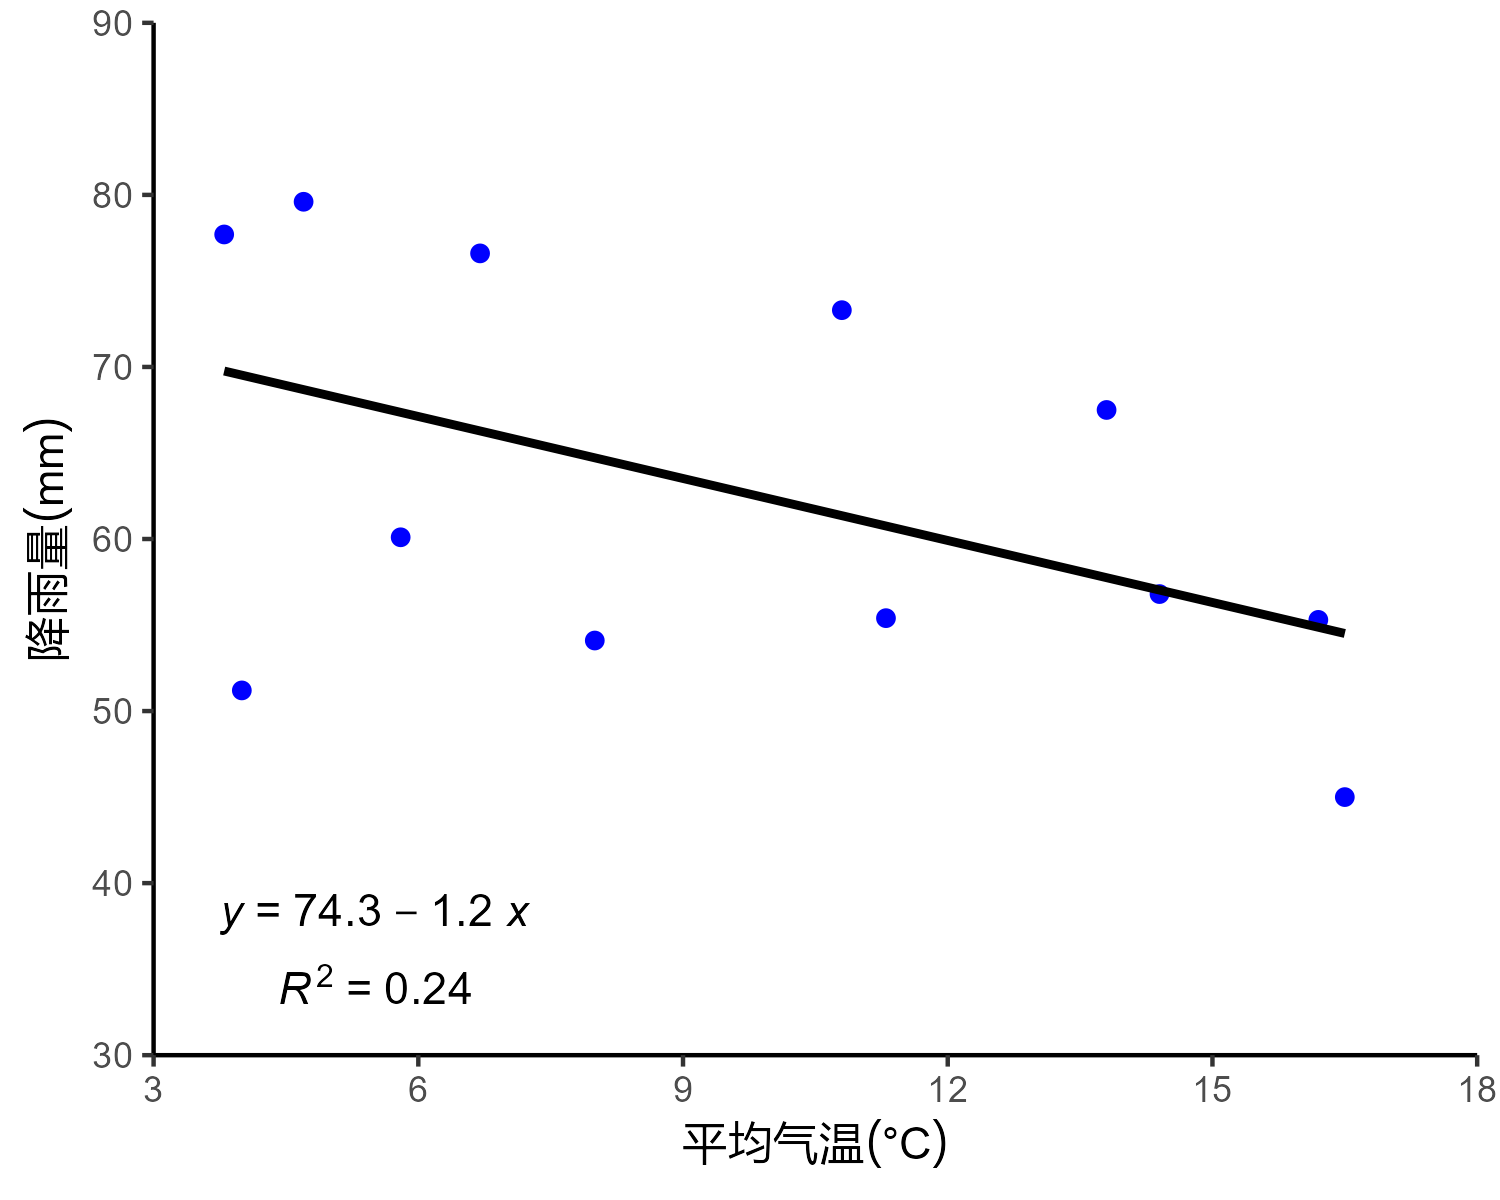
\includegraphics[width=1\linewidth,height=1\textheight]{exp3_files/figure-latex/lm1.png} \end{center}

\section{\texorpdfstring{\texttt{Python}
拟合一元线性回归模型}{Python 拟合一元线性回归模型}}\label{python-ux62dfux5408ux4e00ux5143ux7ebfux6027ux56deux5f52ux6a21ux578b}

\begin{Shaded}
\begin{Highlighting}[]
\ImportTok{import}\NormalTok{ numpy }\ImportTok{as}\NormalTok{ np}
\ImportTok{import}\NormalTok{ pandas }\ImportTok{as}\NormalTok{ pd}
\ImportTok{import}\NormalTok{ statsmodels.api }\ImportTok{as}\NormalTok{ sm}
\ImportTok{import}\NormalTok{ matplotlib.pyplot }\ImportTok{as}\NormalTok{ plt}

\NormalTok{dt }\OperatorTok{=}\NormalTok{ pd.read\_excel(}\StringTok{\textquotesingle{}../data/exp3/3{-}SPSS.xls\textquotesingle{}}\NormalTok{)}
\NormalTok{dt.head()}
\end{Highlighting}
\end{Shaded}

\begin{verbatim}
##    平均气温x/oC  降雨量y/mm
## 0       3.8     77.7
## 1       4.0     51.2
## 2       5.8     60.1
## 3       8.0     54.1
## 4      11.3     55.4
\end{verbatim}

\begin{Shaded}
\begin{Highlighting}[]
\NormalTok{X }\OperatorTok{=}\NormalTok{ dt.loc[:,}\StringTok{\textquotesingle{}平均气温x/oC\textquotesingle{}}\NormalTok{]}
\NormalTok{y }\OperatorTok{=}\NormalTok{ dt.loc[:,}\StringTok{\textquotesingle{}降雨量y/mm\textquotesingle{}}\NormalTok{]}
\NormalTok{X }\OperatorTok{=}\NormalTok{ sm.add\_constant (X)}
\NormalTok{lm\_model }\OperatorTok{=}\NormalTok{ sm.OLS(y,X).fit()}
\BuiltInTok{print}\NormalTok{(lm\_model.summary())}
\end{Highlighting}
\end{Shaded}

\begin{verbatim}
##                             OLS Regression Results                            
## ==============================================================================
## Dep. Variable:                降雨量y/mm   R-squared:                       0.240
## Model:                            OLS   Adj. R-squared:                  0.164
## Method:                 Least Squares   F-statistic:                     3.151
## Date:                  周四, 16 5月 2024   Prob (F-statistic):              0.106
## Time:                        16:15:15   Log-Likelihood:                -44.387
## No. Observations:                  12   AIC:                             92.77
## Df Residuals:                      10   BIC:                             93.74
## Df Model:                           1                                         
## Covariance Type:            nonrobust                                         
## ==============================================================================
##                  coef    std err          t      P>|t|      [0.025      0.975]
## ------------------------------------------------------------------------------
## const         74.3266      7.234     10.274      0.000      58.208      90.445
## 平均气温x/oC      -1.2010      0.677     -1.775      0.106      -2.709       0.307
## ==============================================================================
## Omnibus:                        1.571   Durbin-Watson:                   1.008
## Prob(Omnibus):                  0.456   Jarque-Bera (JB):                0.898
## Skew:                          -0.287   Prob(JB):                        0.638
## Kurtosis:                       1.789   Cond. No.                         25.2
## ==============================================================================
## 
## Notes:
## [1] Standard Errors assume that the covariance matrix of the errors is correctly specified.
\end{verbatim}

\emph{R方为0.2396,说明数据有23.96\%的可能被该回归方程解释,数据与模型的拟合程度较低.}

\emph{由回归方程的F检验可得,\(P = 0.1063 > 0.05\),
F检验无法通过,说明回归方程不显著,自变量不能显著影响因变量.}

\emph{回归模型的方程为 \(y = -1.201x + 74.3266\)
,对自变量进行t检验,\(P_{(x)} = 0.106 > 0.05\),t检验无法通过,说明自变量不能显著影响因变量.}

\end{document}
